\section{Systemarkitektur} \label{ch:Systemarkitektur}

Systemarkitekturen fungerer som udgangspunkt for designfasen af hele systemet.
Den danner overblik over det samlede systemet, hvorved det deles op i mindre blokke. 
De mindre blokke beskriver efterfølgende systemet i nærmere detaljer, således man kan derefter kan gå direkte til design af systemet. For den detaljerede systemarkitektuk henvises til kapitel \ref{P-sec:sysark} \nameref{P-sec:sysark} på side \pageref{P-sec:sysark} i dokumentationen.

\begin{figure}[h]
\centering
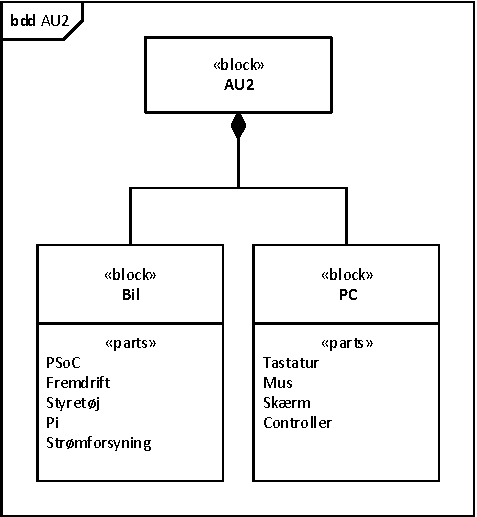
\includegraphics[width=0.55\textwidth]{../fig/diagrammer/bdd_au2.pdf}
\caption{Overordnet BDD for AU2}
\label{fig:bdd_au2}
\end{figure}

På figur \ref{fig:bdd_au2} ses et overordnet BDD for AU2. 
Det ses at systemet AU2 består af en bil og en PC. 
Bilen er her det centrale element i systemet, hvilket kommunikerer med den software der kører på PC'en. 
Denne tilgang er valgt for at kunne fjernstyre bilen med XBox-360 controlleren igennem PC'en over Wi-Fi. På figur \ref{fig:bdd_bil} på side \pageref{fig:bdd_bil} ses et udvidet BDD for blokken Bil.  

\clearpage

\begin{landscape}

\begin{figure}
\centering
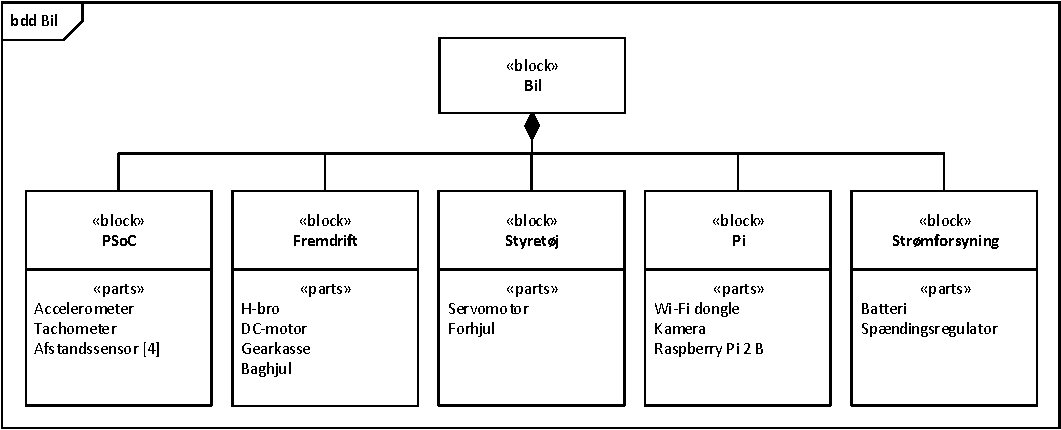
\includegraphics[width=\linewidth]{../fig/diagrammer/bil/bdd_bil.pdf}
\caption{BDD for bil}
\label{fig:bdd_bil}
\end{figure}
\end{landscape}

\clearpage

Formålet med figur \ref{fig:bdd_bil} er at give et logisk overblik over de fysiske dele der er påmonteret bilen. 
Blokkene er opdelt med henblik på deres respektive ansvarsområde i forhold deres funktionalitet. Derfor ses blokkene med tilhørende parts, som herefter kan nedbrydes i moduler til design og implementering.

\begin{figure}[H]
\centering
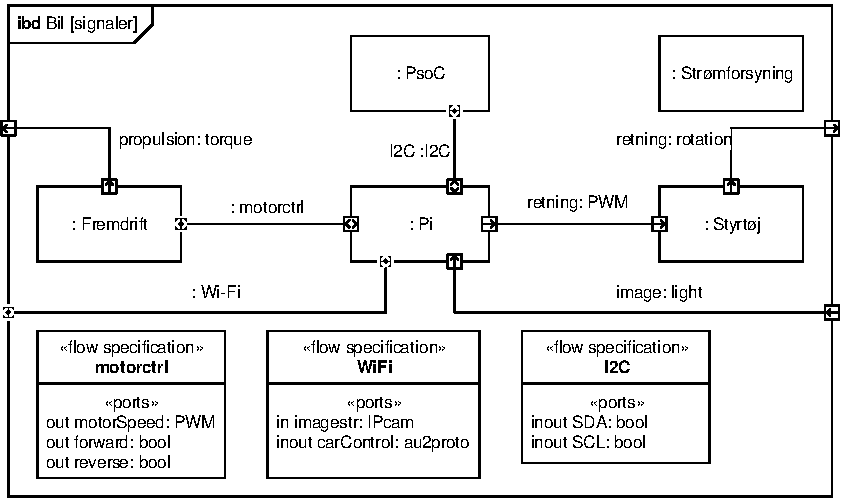
\includegraphics[width=\textwidth]{../fig/diagrammer/bil/ibd_bil.pdf}
\caption{IBD for bil}
\label{fig:ibd_bil}
\end{figure} 

På figur \ref{fig:ibd_bil} ses ibd for blokken Bil. 
Her er beskrevet hvilke signaler der forbinder blokkene samt deres indehold. 
Det ses at blokken \emph{Fremdrift} er forbundet med \emph{motorctrl} som er styringssignalet til motoren.  
I flow-specifications udspecificeres signalernes indehold. 
Diagrammet skal læses i forbindelse med figur \ref{fig:bdd_bil} på side \pageref{fig:bdd_bil}. 

\clearpage